\section{Instrument Signature Removal for DP2 Science Data} \label{sec:isr-science}

Instrument Signature Removal (ISR) is defined by the steps that transform the raw integer image into a floating-point, fully-calibrated image in electron units with an associated variance plane and pixel mask used in downstream data release processing tasks.
Since this process undoes instrument artifacts that enter into the image in the photon transfer chain, it is crucial for the calibration steps to match the physics of the detectors.

Corrections are applied in reverse chronological order relative to the photon transfer chain (Figure~\ref{fig:detector-boxes} in \S\ref{sec:lsstcam:detector-model}).
For example, steps that undo readout-electronics effects therefore appear before steps that undo detector-level effects and additive corrections precede multiplicative ones such as flat-fielding.

Running the processing pipeline with misplaced steps would either apply a correction in the wrong physical units or leave residual structure that invalidates downstream calibrations.
Figure~\ref{fig:isr-pipeline} shows the resulting sequence of corrections as applied to LSSTCam science images for DP2.

\begin{figure*}[t]
    \centering
    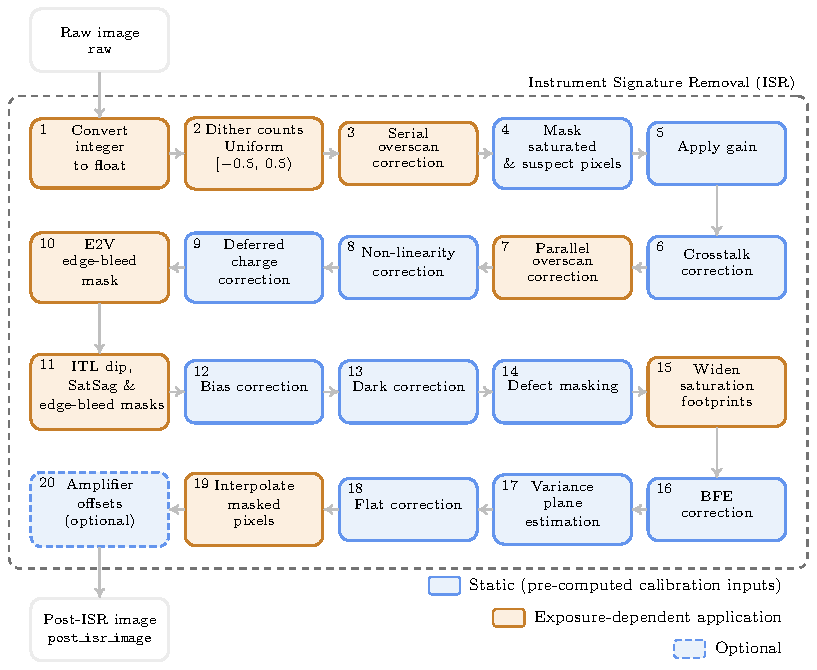
\includegraphics[width=0.9\textwidth]{figures/isr-pipeline.pdf}
    \caption{Outline of the Instrument Signature Removal Pipeline (ISR) applied to LSSTCam science images for DP2.
    The steps in the pipeline follow a very specific sequence determined by the physics of the instrument signature and where it enters in the photon transfer chain.
    Blue boxes denote static ISR steps that apply pre-computed calibration inputs; orange boxes denote steps whose application depends on the science exposure itself (for example, overscan subtraction, dithering, or saturation-footprint growth); white boxes mark the raw input and post-ISR output.
    A dashed border marks a computation rather than an artifact correction (integer-to-float conversion, dithering, overscan statistics, and variance plane estimation).
    The amplifier-offset step remains optional and applies pre-computed per-amplifier offsets when enabled.}
    \label{fig:isr-pipeline}
\end{figure*}

\subsection{ISR Pipeline Overview} \label{sec:isr-science:overview}

The LSSTCam has a particular photon transfer chain and therefore a particular ISR correction pipeline. This pipeline takes in a set of calibrations and a raw image, and it outputs a science-ready image, with complete with a mask plane, provenance, and metadata.

The output exposure's metadata records the calibration epoch, the identifier of the curated collection used, and a per-step record of which ISR corrections were applied or skipped.
This provenance makes it possible to reproduce the processing of any released image, compare products generated across software or calibration versions, and audit the configurations enabled for a given dataset.
The verification, acceptance, and distribution context for these metadata fields is described in \S\ref{sec:verify-accept-certify:data-products}.

The following outline follows Figure~\ref{fig:isr-pipeline} step by step.
Each item names the correction applied, and the reason it sits at this location in the processing chain.

\begin{enumerate}
    \item \textbf{Convert integer to float.}
    Raw images arrive as integer arrays. This first step promotes pixel values to 64-bit floating point precision.

    \item \textbf{Dither counts.}
    A uniform random offset in $[-0.5,\,0.5)$~ADU is added to every pixel.
    This breaks the correlation between true signal and integer quantization before continuous corrections are applied, reducing systematic bias when later steps interpolate, convolve, or divide the image.
    This step is essentially a marginalization step before a full low-signal, differential non-linearity correction can be measured and implemented.

    \item \textbf{Serial overscan correction.}
    An electronic, clock-injected offset plus smaller row-to-row variations are derived from the serial overscan and subtracted from the imaging pixels while the data are still in native analog-to-digital units (ADU).
    Overscan correction must precede gain conversion because the overscan bias is measured and removed in the same units as the raw readout. 
    At this stage we also calculate overscan statistics, including an estimate of the read noise from the scatter in overscan pixels and the amount of deferred charge from EPER statistics.

    \item \textbf{Mask saturated and suspect pixels.}
    Pixels above the PTC turnoff saturation threshold (\S\ref{sec:processing:calibration:ptc}) get flagged as both saturated (``SAT") and suspect (``SUSPECT") in the pixel bit mask before further signal corrections.
    Early masking prevents corrupted or non-physical pixel values from biasing downstream estimates that assume a well-behaved signal.

    \item \textbf{Apply gain.}
    Per-amplifier gains derived from the PTC (\S\ref{sec:processing:calibration:ptc}) convert pixel values from ADU to electrons.
    Electron units are the native domain for deferred-charge modeling, BFE correction, and variance plane estimation, all of which were calibrated assuming a linear conversion from measured counts to stored charge.

    \item \textbf{Crosstalk correction.}
    Electrical coupling between adjacent amplifier outputs is removed using the crosstalk matrix (\S\ref{sec:processing:calibration:xtalk}).
    Crosstalk is applied after gain conversion so that coupled signals are corrected in electron units, consistent with how the matrix was measured.

    \item \textbf{Parallel overscan correction.}
    Analogous to the serial overscan step, the parallel overscan region provides a column-direction estimate of readout offset that is subtracted from the imaging area.
    It follows crosstalk correction because amplifier coupling can inject signal into overscan regions, and removing crosstalk first yields a cleaner overscan bias estimate.

    \item \textbf{Non-linearity correction.}
    The double-spline linearizer (\S\ref{sec:processing:calibration:linearity}) maps measured counts to a linearized electron count by subtracting absolute and amplifier-relative spline corrections.
    This step must precede deferred-charge correction because the deferred-charge model and its calibration were fit assuming that signal-dependent readout non-linearities have already been removed (\S\ref{sec:processing:calibration:cti}).

    \item \textbf{Deferred charge correction.}
    Residual charge left in pixels during serial readout---from global charge transfer inefficiency, local electronic offset in the output amplifier, and serial charge traps on ITL sensors---is corrected using the parameters fit in \S\ref{sec:processing:calibration:cti}.
    This step sits late in the readout-electronics portion of the chain because deferred charge is imprinted during serial transfer, after non-linearities in the output path have acted on the signal.
    We do not correct deferred charge on E2V sensors because the deferred charge level is already below the level defined by \citet{LPM-17}.

    \item \textbf{E2V edge-bleed mask.}
    We flag the ``SAT'' mask plane bit for pixels in E2V amplifiers that show uncorrectable charge spill from bright regions at the serial-register edge.
    
    \item \textbf{ITL dip, SatSag, and edge-bleed masks.}
    We flag the ``ITL\_DIP'' mask plane bit for pixels in ITL amplifiers that exhibit a pixel column depression in response near certain amplifier boundaries (the ``ITL dip''), a sag in apparent signal after saturation (``SatSag''), and edge bleeding analogous to the E2V case.
    These vendor-specific masks follow deferred-charge correction because the artifacts they mark are readout- and saturation-related structures that should be evaluated on linearized, CTI-corrected data.

    \item \textbf{Bias correction.}
    A combined bias frame (\S\ref{sec:processing:calibration:bias}) is subtracted to remove the fixed-pattern electronic offset that remains after overscan subtraction.
    Overscan correction handles the spatially static electronic structure imprinted in the images before charge readout.

    \item \textbf{Dark correction.}
    The combined dark frame (\S\ref{sec:processing:calibration:dark}), scaled by the science exposure time, is subtracted to remove thermal dark current accumulated during exposure integration.
    Dark correction follows bias subtraction because both are additive offsets, and the dark frame is constructed from bias-subtracted dark exposures.

    \item \textbf{Defect masking.}
    Persistent bad pixels, columns, and other static defects identified during calibration (\S\ref{sec:processing:calibration:defects}) are merged into the pixel mask.
    Applying the defect mask after deferred-charge, bias, and dark correction places it once readout-electronics effects and integration-period offsets have been removed, matching the processing state in which the defect catalog was built and ensuring that later defect footprint widening and interpolation operate on the full static bad-pixel map.

    \item \textbf{Widen saturation footprints.}
    The saturation mask is expanded spatially to include pixels affected by charge spill and trails from saturated sources.
    This step follows defect masking so that all static bad regions are known before the saturation footprint is grown into neighboring pixels.

    \item \textbf{BFE correction.}
    The electrostatic BFE (\S\ref{sec:processing:calibration:bf}) redistributes flux among neighboring pixels to undo charge-cloud repulsion in the silicon.
    In the photon transfer model (Figure~\ref{fig:detector-boxes}), the BFE is the earliest detector-level effect on incident photons, so its correction appears correspondingly late in ISR.
    It is applied after the image has been converted to linearized electron units and after additive calibration-frame corrections.
    The correction also needs to match the boundary-shifts, which were also calibrated from PTC covariances measured after these corrections.

    \item \textbf{Variance plane estimation.}
    An expected variance is assigned to each pixel using the PTC-derived gain and read noise (\S\ref{sec:processing:calibration:ptc}).
    The variance plane is computed after gain application and BFE correction so that it reflects the electron units and pixel correlations relevant to source detection and weighting in downstream analyses.

    At this stage the expected per-pixel variance follows the Poisson-plus-read-noise model
    \begin{equation}
        \sigma^2_{ij} = \frac{F_{ij}}{g_a} + \left(\frac{\sigma_n(a)}{g_a}\right)^2,
        \label{eq:isr-variance}
    \end{equation}
    where $F_{ij}$ is the science image value in the current ISR units, $g_a$ is the PTC gain for amplifier~$a$ (electrons per ADU), and $\sigma_n(a)$ is the read noise in electrons.
    For DP2 science processing the image is already in electron units, so $g_a = 1$ and Eq.~\ref{eq:isr-variance} reduces to $\sigma^2_{ij} = F_{ij} + \sigma_n(a)^2$.
    Pixels with non-positive variance are flagged in the mask.
    
    Since the variance plane is used to estimate the uncertainy on just the charge acculumated in the image, it needs to be computed before flat-field correcting.

    \item \textbf{Flat correction.}
    The normalized flat field (\S\ref{sec:processing:calibration:flats}) is divided into the image to correct pixel-to-pixel variations in quantum efficiency and optical throughput.
    Flat-fielding is intentionally late in the pipeline: it is a multiplicative correction that must be applied only after all additive electronic and dark offsets have been removed, so that the flat field encodes relative sensitivity rather than residual bias structure.

    \item \textbf{Interpolate masked pixels.}
    Pixels in the ``SAT'', ``BAD'', and ``UNMASKEDNAN'' mask planes are filled by interpolation from neighboring unmasked values; ``SUSPECT'' pixels are flagged but not interpolated by default.
    Interpolation is performed after flat-fielding so that both the science signal and the replacement values are in the same calibrated flux units expected by algorithms that assume a continuous image (for example, background estimation and certain astrometric measurements).

    \item \textbf{Amplifier offsets (optional).}
    Small per-amplifier additive adjustments derived from flat-field residuals may be applied as a final optional step to reduce residual flux discontinuities at amplifier boundaries.
    This step is optional because the PTC gain solution already includes average amplifier matching (\S\ref{sec:processing:calibration:ptc}); the offset correction addresses any remaining channel-to-channel offsets visible after the full ISR chain.
\end{enumerate}
